%==============================================================================
% Mini Preamble.
%==============================================================================

\documentclass[11pt]{article} % 10pt article, want AMS fonts.
\makeatletter					% Make '@' accessible.
\pagestyle{myheadings}				% We do our own page headers.
\skip\footins=4ex				% Space above first footnote.
\hbadness=10000					% No "underfull hbox" messages.
\makeatother					% Make '@' special again.
\usepackage{fullpage}
\usepackage{graphicx}
%==============================================================================
% Title.
%==============================================================================

\begin{document}
\centerline{\LARGE{CSCI 2951-F Final Project}}
\centerline{Enrique and Ellis and Kavosh and Dave}
\vspace{2mm}


% --- SECTION: Paper Overview ---
\section{Paper Overview}

Note: Introduce the problem that they're solving, i.e. identify the main research contribution made (a natural language version of theorem 1 ish? that there is this relationship between model accuracy and planning depth, and that gamma lets you control that).


% --- SECTION: Domains ---
\section{Domains}

% Section: Rock Sample
\subsection{RockSample}

% Section: Randomized MDPs
\subsection{Randomized MDPs}



% --- SECTION: Hypotheses ---
\section{Hypotheses}

% Subsection: Figure 6
\subsection{Figure 6}

% Subsection: Figure 7
\subsection{Figure 7}


% --- SECTION: Experiments ---
\section{Experiments}

Idea: Discuss how we chose to implement our version of the experiments?



% --- SECTION: Results ---
\section{Results}

Summary of their results, summary of our results.

Cross validation with RandomMDP
$$\begin{tabular}{cc}
	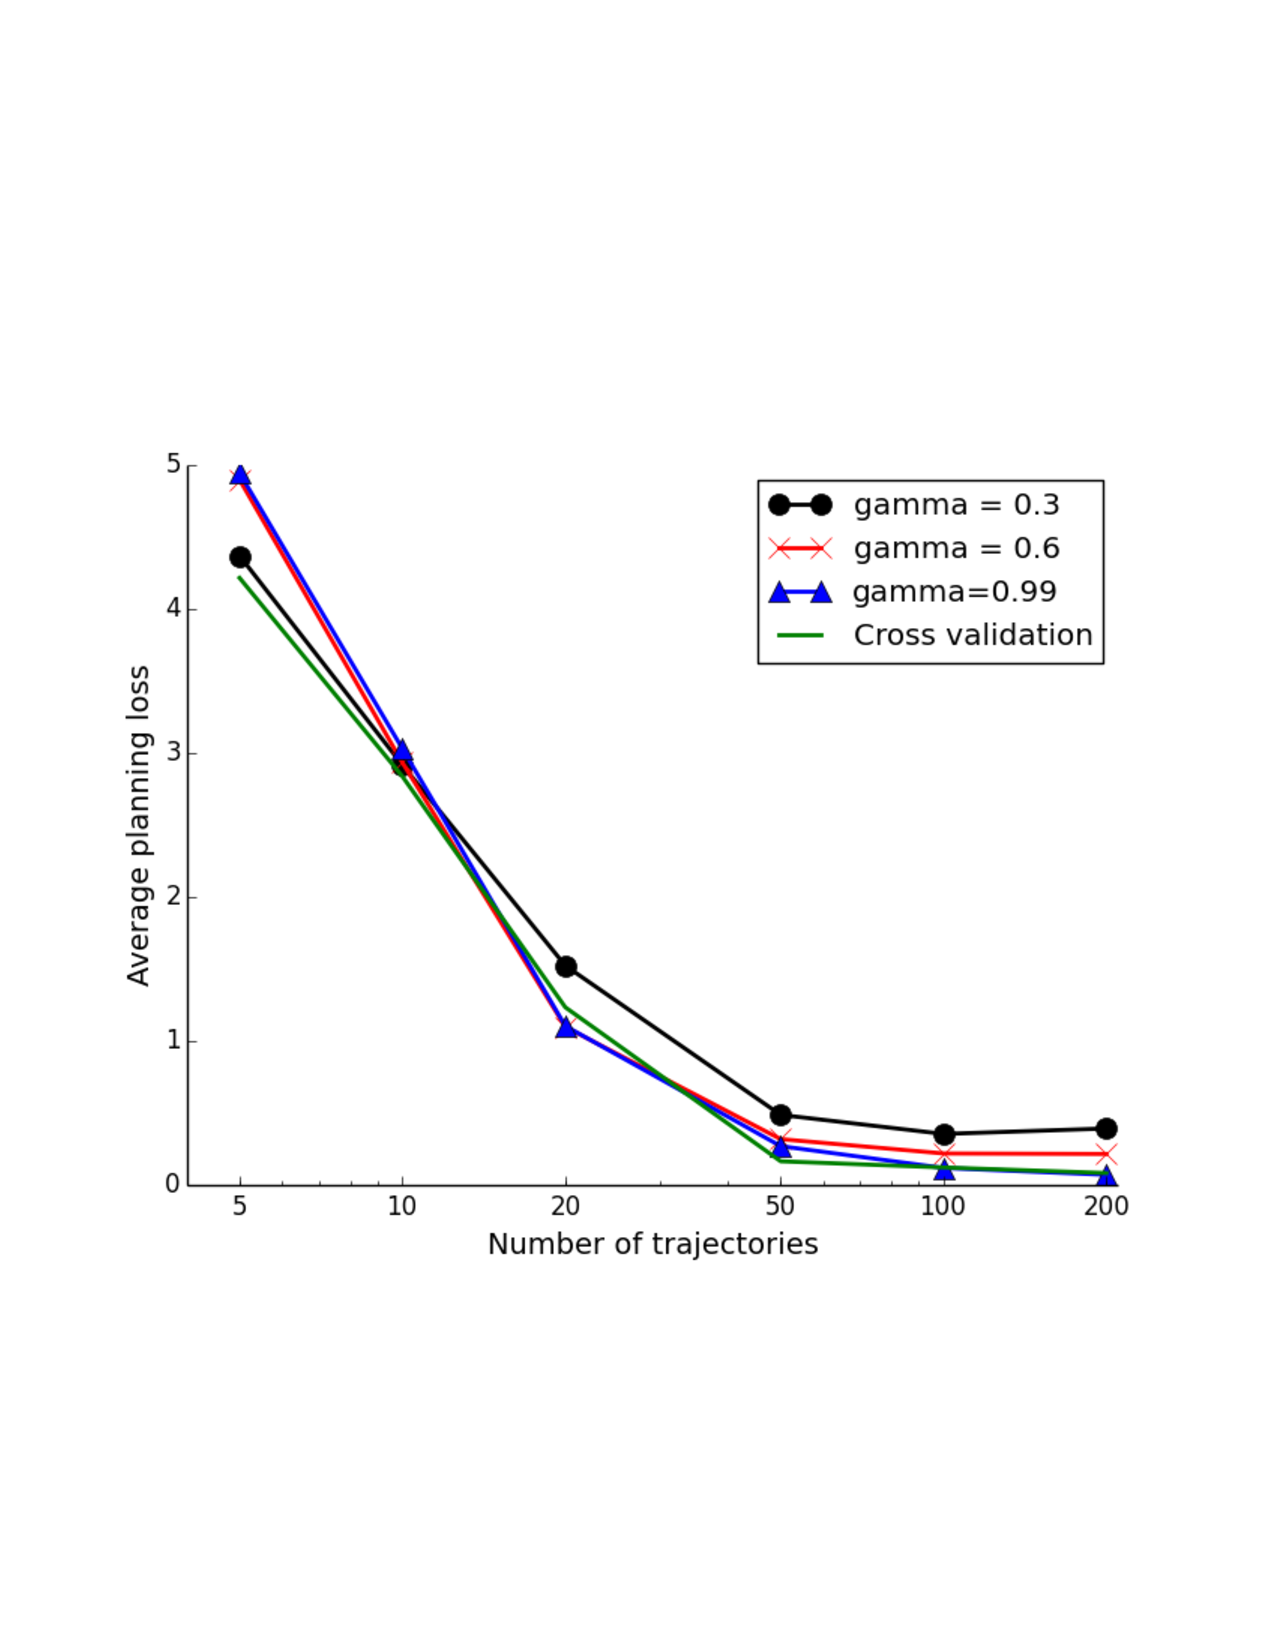
\includegraphics[page=1,width=.5\textwidth]{../results/figure_2.pdf} &
	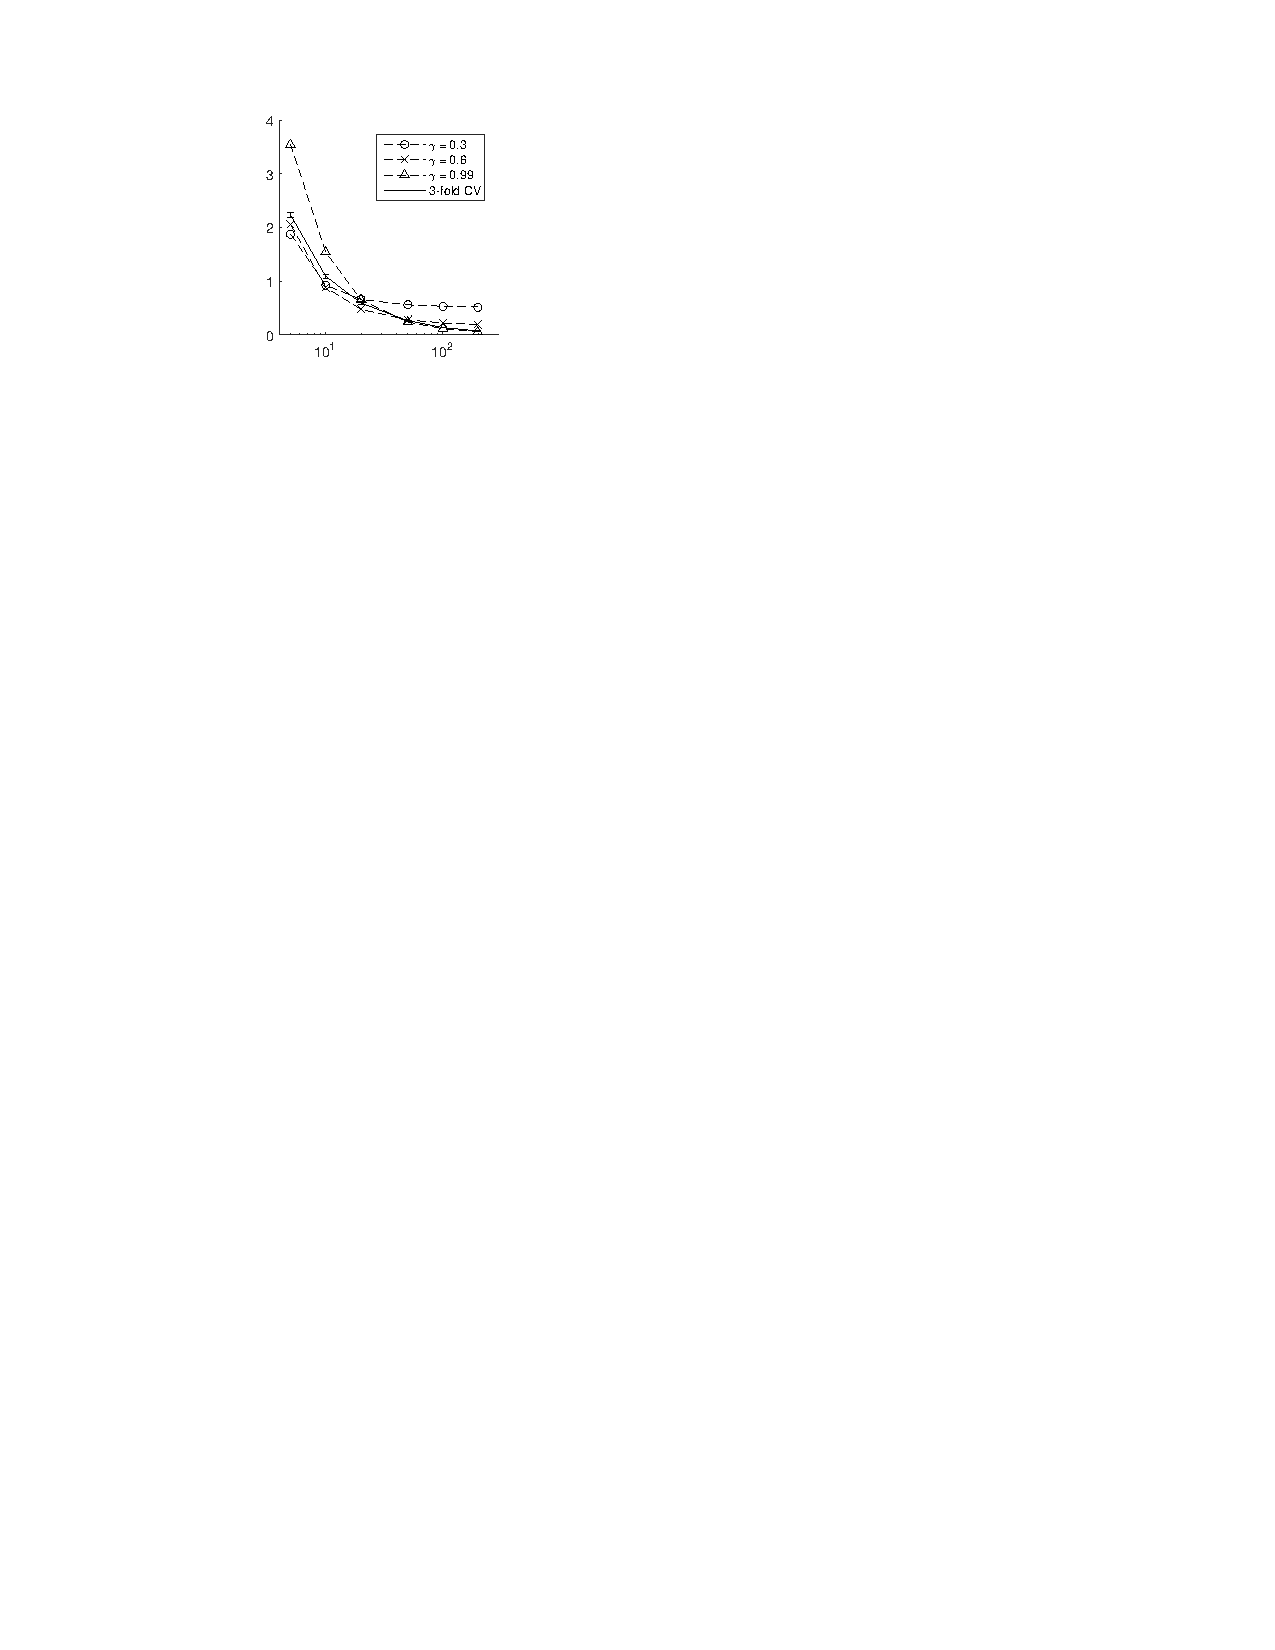
\includegraphics[page=1,width=.41\textwidth]{../results/originalCV.pdf}\\
	our results & their results \\
\end{tabular}$$


% --- SECTION: Reproducibility Discussion ---
\section{Reproducibility Discussion}

Discussion of how reproducing results was difficult, what assumptions we made, what parameters and other bits of info were left from the paper.

For the RockSample:
\begin{itemize}
\item Actual values of UCT exploration bias
\item Gamma
\item Treatment of POMDP with UCT (belief MDP?)
\item Initial state? Randomized? Fixed? Actually super important
\item Initial configuration of rocks?
\end{itemize}


% --- SECTION: Conclusion ---
\section{Conclusion}


% --- BIBLIOGRAPHY ---
\bibliographystyle{acm}
\bibliography{lsdm_final}

\end{document}